\chapter{Literature Review}
  \section{Space Exploration and NASA's Journey to Mars}
    \subsection{A Brief History}
      The human race possesses a trait that proposedly sets us apart from the majority of life forms around us; the powerful will to explore what is unknown. It is the curiosity and the thrill to push past the boundaries of what is thought to be possible, perhaps felt stronger by some, that forms the basis of many scientific endeavours relating to facts of life and existence around and outside of the immediate environment in which we live.
      
      A prime example of such a drive to explore is in the research and exploration of outer space, which, from a technological perspective, transitioned from astronomer's dream to scientist's and engineer's reality during the Cold War. Although space exploration as we know it today is motivated by human curiosity, it was during this period of political tension that significant breakthroughs in spacecraft and rocket propulsion technology were brought about. This period is referred to as the ``Space Race'' and stemmed from research and development of nuclear weaponry during World War II \cite[p. 147]{cornwell2003hitler}. The race began with the attempted launches of artificially made satellites \cite[pp. 3-5]{schefter1999the} and within the 40 years following the success of the USSR's \textit{Sputnik I} in 1957, the first object to be put into orbit by man, space technology progressed from early manned flights beginning in 1961\footnote{First human in space, Soviet launched} through the \textit{Apollo 11} lunar flight to having flown by of the majority of the planets in our solar system.
      
      By 1981, the launch of \textit{Columbia} \cite{williamharwood2009}, a space shuttle designed to be used for more than one flight, marked the beginning of reusable space technologies answering to the problem of cost and with the forethought of future increase in space flight frequency and demand. Today, the efforts to lower the cost of space travel and the attempt to bring space exploration into the private sectors to make these opportunities more realisable by the public are evident in Elon Musk's SpaceX development of the Falcon 9, a reusable rocket that returns and lands safely back on the surface of Earth \cite{spacex_popularmechanics}.
      
      The National Aeronautics and Space Administration (NASA) of the United States has been and still is responsible for a large chunk of mankind's search among the stars and, with respect to research and exploration, has made great efforts to better understand the planet that we live on in conjunction with the immediate spacial environment around Earth, the solar system and the planets within, and that which lies in deep space. After the Apollo lunar missions, efforts by NASA to explore involved one of the first space stations, the \textit{Skylab}, which suffered technical difficulties originating from launch but proved the ability to conduct research in space as well as allow astronauts to perform repairs and maintenance to artificial bodies in that environment \cite{compton1983living}. \textit{Skylab} was followed by the International Space Station (ISS), intended to be a more sustainable microgravity environment in which to conduct research that might require such conditions. Research of this type include a very broad range of investigations from the effects of near-weightlessness on plants and animals through to growth of human-like tissues and protein crystallisation \cite{nasaresearch}. An area of research that specifically relates to this project is in the development of technology to allow for longer, cheaper and faster flights in space, both in spacecraft materials and systems and in astronaut health and performance. This is closely coupled with the search by entities around the world for other forms of life outside of Earth's atmosphere fuelled by the prospect of finding environmental architectures similar to ours. One of NASA's goals outlined in \cite{nasa2010act} is to send humans to Mars and this has lead to enormous amounts of research, promising engineering and technological successes that will ultimately allow humankind to extend civilisation across more than one planet.
    
    \subsection{Mars} 
      NASA has identified that Mars is a planet with greater similarity in formation and conditions in its history and as a result has been a target of exploration for more than 40 years. This has involved multiple flybys and orbits starting from 1962 through to the first lander, the \textit{Viking 1}, to touch down on the surface of the planet in 1975 \cite{marsprogram2008}. NASA's Jet Propulsion Laboratory (JPL) landed the spacecraft, named \textit{Pathfinder}, that contained the first successful rover vehicle, the \textit{Sojourner}, in 1997 \cite{pathfindersojournerjpl}. The purpose of this mission was to prove the possibility of cheaper spacecraft development and the transport of scientific equipment to the planet as well as taking photographs of the red surface, from the surface. 
    
    
    % TODO: NASA and Mars
    % Something about why we need rovers and what was NASA's goal etc
    
  \section{The Mars Science Laboratory and Curiosity}
    \subsection{Overview}
      The Mars Science Laboratory (MSL) is a mission that was launched by NASA to further explore the surface of Mars, one of many orbiter, lander and rover type missions as part of the Jet Propulsion Laboratory's (JPL\footnote{Jet Propulsion Laboratory of California Institute of Technology}) Mars Exploration Program (MEP). The program is structured to work towards a set of goals to ultimately understand and determine the potential for life on Mars \cite{meptheme} by observation of the current climate and geology. The MSL is the latest mission in operation as part of MEP and was intended to span roughly one Martian year after touchdown on Mars. However, it has continued to operate for more than double that amount of time. 
      
      \begin{figure}[ht]
        \centering
        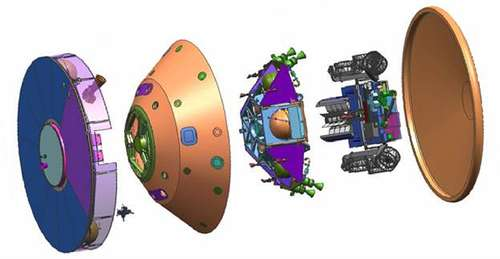
\includegraphics[width=0.7\textwidth]{figures/mslSpacecraftExplodedView.jpg}
        \label{fig:mslSpacecraftExplodedView}
        \caption{An exploded 3D model of the Mars Science Laboratory spacecraft including the cruise stage (far left) and heat shield (far right) \cite{fig:mslSpacecraftExplodedView_cite}}
      \end{figure}
      
      
      MSL was launched from Cape Canaveral Space Station, Launch Complex 41, atop an Atlas V vehicle, a two stage rocket \cite{harwood2014sfn}. The mission required the launch vehicle to insert the five-piece MSL spacecraft into a transfer orbit in a process known as a Trans-Mars Injection (TMI) allowing the spacecraft to arrive at Mars after a 566 million kilometre trip that lasted 256 days. Figure~\ref{fig:mslSpacecraftExplodedView} shows a 3D render of the components of the spacecraft that made the trip. Four trajectory correction manoeuvres were made during the flight to result in a landing near ``Mount Sharp'' in Gale Crater, deemed the most accurate landing on Mars of any other spacecraft \cite{martinmur}.
      
      % TODO: Launch site choice
    
    \subsection{Primary Mission Goals and Objectives}
      Touching down on the surface of Mars, the MSL had primary objectives tailored to contribute to the four goals as outlined in the MEP. The objectives were carried out by the MSL's flagship component, the Curiosity rover, and consisted of a wide range of biological and geological observations such as to determine the chemical building blocks that exist on the surface including organic carbon compounds, prospective historical biological activity, atmospheric processes of evolution, surface radiation and state and distribution of water \cite{mslobjectivesjpl}.
      
      Apart from the primary objectives, the MSL mission pushes further the boundaries of space exploration in that it proved the ability to land heavier vehicles at incredibly precise landing accuracy as well as the achievement of wider surface coverage to collect and observe more diverse samples of the surface of Mars.
              
    \subsection{Curiosity Technical Breakdown}
      23\% of the MSL spacecraft's total mass of 3.893 metric tonnes was thanks to the missions vehicle, \textit{Curiosity}. The six wheeled, instrument-bearing rover features much improved hardware over previous vehicles along with a multiple systems of new instruments to enable the carrying out of the mission objectives.
      
      The mechanical and technological specifications are broken down in the sections that follow.
      
      \subsubsection{Mechanical Structure}
        Structurally, \textit{Curiosity} comprises of mechanical features and principles borrowed from the previous three rovers, \textit{Sojourner}, \textit{Spirit} and \textit{Opportunity}, however, was made much larger (almost double the size). The reason behind the increase in size was the need for extra volume in which to fit the significantly larger set of scientific instruments, 100 times larger than the suite on \textit{Sojourner} \cite{planetary2011}.
        
        ![Body structure image]
        
        The body of the rover, a shallow, rectangular box, dominates its structural layout and serves as the central feature onto which all others subsystems are mounted. The chassis is also host to some of the rover's scientific instruments as well as the avionics box. The electronics that make up the avionics operate in a warm environment \cite{nasajulypresskit}, thus requiring the body to provide thermal insulation from the external conditions of Mars, giving it the name the Warm Electronics Box (WEB). The regulation of internal temperature, aided by the use of electrical heaters, is taken care of by a heat rejection system involving a pumped-fluid loop with the source of heat being the power generator, discussed in a section to follow. Thermal regulation also widened the range of potential landing sites with respect to their distance from the equator.
        
        Overall, \textit{Curiosity} was designed to exceed normal standards of mechanical robustness given the fact that hand-on maintenance is not a possibility when operating so far away from Earth. All subsystems on the rover minimised the opportunity for accidental collisions that might result in unfixable damage to the subsystems and thus jeopardy of the entire mission. In addition to the stringent design procedures, complex simulations of the rover's mechanical operation were done in virtual environments which allowed engineers to ensure, as far as possible, the success of the design in the differing environment that is on the surface of Mars.
        
      \subsubsection{Manoeuvrability}
        One of the main similarities between \textit{Curiosity} and its predecessors is the mechanical subsystem that provides the rover's ability to move around the surface of the planet. The six wheels, each half a meter in diameter, are constructed from aluminium with titanium spokes specially designed to allow for an amount of flexibility required for shock absorption and support. Protruding from the skin of the wheels are cleats in the shape of chevrons. This is an improvement over previous rovers where the cleats were horizontal, a flawed design in that sideways slippage was possible. The angled nature of the chevron cleats on the wheels of the \textit{Curiosity} aimed to prevent this motion. The thin, tubeless design allowed the wheels to be as light as possible which is important not only for driving on soft parts of the Martian landscape (termed ``floating''), but also for the unique landing sequence the rover had to carry out. The significant increase in the total weight of \textit{Curiosity} meant that conventional means of landing, such as the use of air-cushion support, was not possible. The MSL leveraged the mechanical suspension subsystem on its rover for touchdown instead of providing a separate lander itself. Here, the springy wheel design helped minimise the damage brought about by the impact. As far as weight minimisation of the wheels was concerned, during the moments before the rover was released to land on the surface, the wheels were deployed in a dynamically stressful fashion from their folded position kept during flight. The deployment was sudden and extra weight would have increased the already significant forces imparted on the suspension subsystem during this manoeuvre \cite{planetary2014}.
        
        However, the feature that is definitive of current and previous Mars mobility systems is the structural arrangement of the wheels in the mechanical suspension subsystem. Each wheel is mounted to an end of the mechanical linkage designed based on the ``rocker-bogie'' principle. On each side of the rover, the linkage consists of two pivoting beams, one mounted to the side of the rover body, named the ``rocker'' and the other mounted to the middle-facing end of the rocker, called the ``bogie''. The front-facing end of the rocker and both ends of the bogie each host a wheel structure which consists of a pivot and strut for the front and rear wheels and a strut for the middle wheel. Both mount points allow for rotation of the beams such that, to a certain extent, the linkage as a unit remains level despite uneven terrain. This means that any of the three wheels on a side of the rover may lift due to an obstacle, up to the size of the wheel itself, without any of the other wheels lifting off the ground. This results in the obvious benefit of a maximisation of stability, minimisation of angular displacement of the rover body and maximisation of wheel contact with the surface of Mars. Figure~![] shows one of the sides of the mobility system.
        
        ![RockerBogie image]
        
        In addition to the freedom of movement of each wheel, the rocker beams from both sides of the rover are connected via a differential bar mounted atop the rover body. The bar, which pivots about a central point on the deck of the body, limits the relative movement of the rocker beams such that one rocker will rotate absolutely in the opposite direction of the other. This significantly reduces the amount of tilt and pitch the body experiences when wheels on one corner of the rover are lifted above the other corners as well as maintains even load across all wheels. In addition, the differential provides the second axis of stability needed to keep the body from toppling forward or backwards about the rocker pivot points.
        
        All six wheels have drive motors that may act independently with each motor mounted to a strut. The four corner wheels' struts are connected to a pivot, actuated by a highly geared motor to allow independent rotation for steering. The configuration allows for \textit{Curiosity} to turn conventional arcs as well as turn on the spot, an advantage for its mobility. Priority was not placed on speed for the drive motors but rather they were designed to provide high torque for robustness and for travelling on Martian terrain. The maximum speed of \textit{Curiosity} is approximately 4 centimetres a second \cite{msllegsandwheels}.
        
        The mechanical mobility systems are coupled with the advanced navigational system aboard the rover, a pairing between an arrangement of navigational cameras and software. Four pairs of black and white ``Engineering Hazard Avoidance Cameras'' (Hazcams) with a field of view of approximately 120 degrees are positioned at the lower front and rear of the rover body, providing the rover with awareness of obstacles. The pairs of cameras create 3-dimensional maps of the terrain in front of and behind the rover. Together with the aid of this environmental mapping, two additional pairs of cameras with a much narrower field of view, namely the ``Engineering Navigation Cameras'' (Navcams), are mounted to the mast of the rover to provide a complementary perspective of the terrain.
             
      \subsubsection{Rover Compute Element}
        At the heart of \textit{Curiosity} is the computational entity responsible for control of all systems on-board the rover as well as facilitation of communications with the team on Earth. This set of pairwise redundant computers is called the ``Rover Compute Element'' (RCE) which contains more memory than previous rovers and is hardened against the effects of radiation from the outside environment. The RCE makes use of a \textit{RAD750} CPU designed by IBM and manufactured by BAE Systems Electronics, the radiation-hardened version of the \textit{PowerPC 750}. The \textit{RAD750} has a clock frequency of 110-200 MHz providing more than 266 MIPS of processing power. The pair redundancy of the RCE is such that one of the ``sides'' of the RCE is operating at a time while the other side kept in ``cold backup''. A software feature named ``second chance'' was built into the system whereby the alternate side of the RCE could take over basic control during the critical moments of the MSL's entry, descent and landing should the primary side fail \cite{nasajulypresskit}. During the flight to Mars, multiple versions of the entry, descent and landing software was sent to the spacecraft as improvements to the complicated procedure. After the landing, the original software was replaced by one which included control of the rover specifically on and around the surface of Mars. The RCE did not have enough memory to accommodate both flavours of the governing software and as such, each was installed at different points during the mission \cite{cnn2012milesoff}.
        
        The RCE software involves the use of a real-time operating system (RTOS) approach to core scheduling and operation. JPL opted for a COTS solution for the RCE software and used an RTOS product from Wind River Systems called VxWorks. The operating system was first released in 1987 and has been used in multiple industries from space and defence to consumer electronic and automotive applications \cite{electronicsdesign2011vxworks}, not to mention having been a part of 20 previous JPL's missions. Over the years, VxWorks has been improved in areas of modularity and upgradeability and offers a wide variety of application layers aimed at the Internet of Things. The choice by JPL to, yet again, use VxWorks on the RCE was motivated by its reliability, maturity, an extensive set of supporting tools and low-level scheduling hooks for critical real-time operations \cite{extremetech2012insidecuriosity}.
        
      \subsubsection{Additional Internal Systems}
        Stemming from the central control principle of the RCE are other computing and sensory subsystems that monitor and maintain healthy operation of the rover. One of these systems is the Inertial Measurement Unit (IMU) which gives \textit{Curiosity} a rotational awareness about three axes: roll, pitch and yaw. It is used with the acquired 3D map of the rover's immediate surroundings to estimate the angular position of the rover during navigation and thus ensure that the rover is stable and safe.
        
        \textit{Curiosity} also has an internal control subsystem that monitors various measurements including temperature, power consumption, power storage and communication systems. The control loop will ensure that the rover remains operational and can produce warnings should any of the measurements be abnormal.
               
      \subsubsection{Communication}
        Communication with the rover from the ground station on Earth is arguably the most critical component of the mission besides the rover itself. It allows the upload of series of commands generated by the team together with the software here on Earth as well as the download of scientific data, rover telemetry and images to aid the team in keeping the rover geographically aware. The communication systems were designed to be redundant and to ensure good quality links despite challenges involving the Earth's and Mar's rotation about their own axes and obstructions as a result. Figure~\ref{fig:litreview-telecomsstructure} shows a depiction of the telecommunication system structure.
        
        \begin{figure}[h]
          \centering
          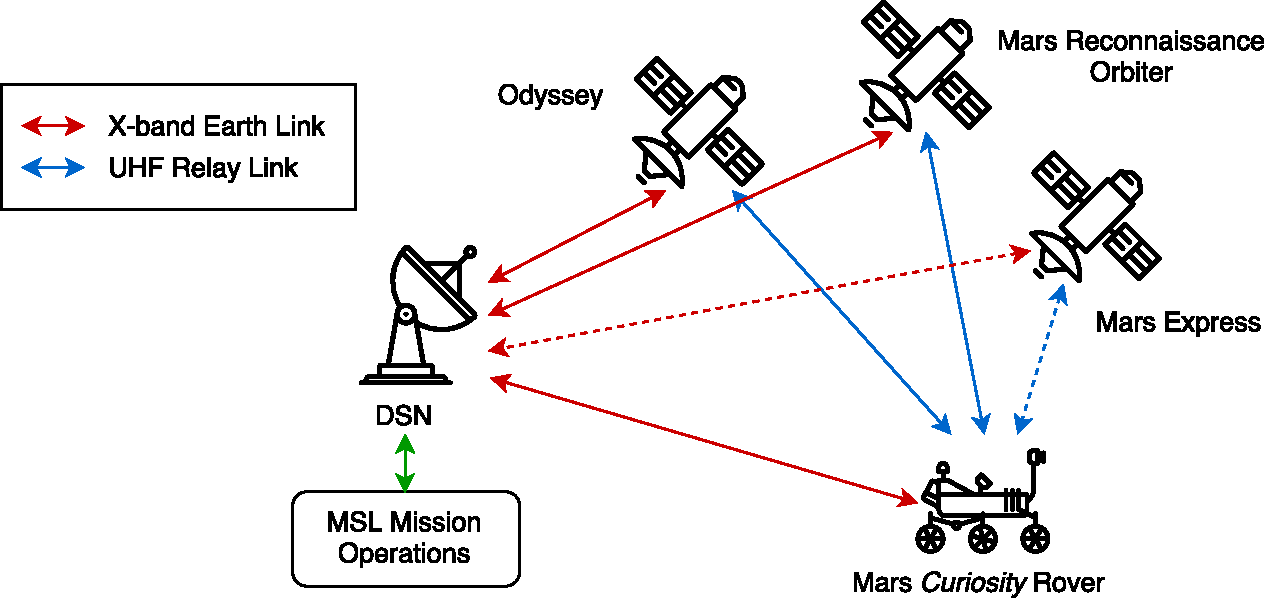
\includegraphics[width=0.71\linewidth]{figures/litreview-telecomsStructure}
          \caption[Diagram showing the structure of the MSL telecommunications system]{Diagram showing the structure of the MSL telecommunications system. Adapted from \cite{fig:litreview-telecomsstructure_cite}.}
          \label{fig:litreview-telecomsstructure}
        \end{figure}

        
        The Earth based component of this communication link originates from a collection of large antennas placed strategically around the Earth that alongside performing astronomical observation, provides communications for spacecraft that are travelling at an interplanetary scale. The system, a part of JPL, is called the NASA Deep Space Network (DSN) which consists of three facilities positioned in California, Spain and Australia \cite{jpldsnabout}. The positioning of the antennas in this way allows effective communication irrespective of the angular position of the Earth, meaning longer contact time between the team on Earth and \textit{Curiosity}. For JPL, the DSN is close to home and thus mainly hosts the central data hub for communications with the rover.
        
        On the Martian side of the link, the rover has aboard three antennas, two of which support the X-band\footnote{X-band - a radio frequency band (between 8.0 and 12.0 GHz) within the microwave region used for engineering communication and radar} communication frequency and a third for Ultra-High Frequency (UHF) software radio communication. The X-band telecommunication system gives the rover a direct communication connection between Mars and the DSN on Earth and consists of a high-gain antenna (HGA) and the Rover low-gain antenna (RLGA) \cite{jpltelecom}. The HGA is movable with two degrees of freedom allowing \textit{Curiosity} to point it accurately back at Earth. This antenna facilitates direct to Earth (DTE) command transmission and direct from Earth (DFE) telemetry at between 160 bps and 800 bps depending on the DSN station size. The RLGA is used mainly for contingency DFE commands and is kept as more of a redundant communication feature. Downlink communication via the RLGA is also possible but again used in case of primary communication failure.
        
        The main method of communication with the rover when on the surface of Mars, however, is via the UHF system which uses the currently operational Mars orbiter spacecraft, the Mars Reconnaissance Orbiter (MRO) and Odyssey, as relays to the DSN. Relaying communication via multiple spacecraft which are orbiting the planet means that less power for signal amplification is required from the rover itself and the time of coverage from the perspective of the DSN stations is increased because objects orbiting the planet are obstructed by the planet body for shorter periods of time. MRO is the primary relay and Odyssey remains the redundant relay for when MRO is unavailable, provided the significantly lower data transfer speed allowed data transfer within DSN time and UHF energy constraints.
        
      \subsubsection{Instrumentation}
        Scientific observation and investigation of the surface of Mars by the \textit{Curiosity} rover forms the crux of the MSL mission and the instruments aboard the rover are the tools with which JPL and NASA are doing such. The ten instruments, primarily scientific, hosted by the rover body, are each designed to perform specific tasks on different aspects of the rover's surroundings and samples from which it may acquire. The typical flow of investigation would be initiated by inspection of high resolution images from the rover's array of cameras. Features of interest are then located, navigated to and further inspected by the instruments mounted on the rover's robot arm and hand. Features may be inspected using those tools, or brought into the rover's body for further analysis, should that be required. Additionally, atmospheric features may be observed using the instruments design for these types of investigations.
        
        The range of instruments, as highlighted by the flow of investigation above, are split into four categories based on their method of contact with their subject. The list below shows the classification as mentioned and provides a short summary of each of the instruments.
        
        \begin{itemize}
          \item \textbf{Remote Sensing Instruments}
          \begin{itemize}
            \item \textit{Mastcam (Mast Camera)}: a suite of two fixed-focal length (FFL) cameras, one the Narrow Angle Camera (NAC) with a $5.1^{\circ}$ FOV and 100 mm focal length, and the other the Medium Angle Camera (MAC) with a $15^{\circ}$ FOV and a 34 mm focal length \cite{mslsciencecornermastcam}. Each camera contains 8 Gb of buffer memory able to store over 5 500 raw frames, as well have the ability to pass the images through a collection of filters. Both cameras, although different in their FOV, focal length and color filter specifications, were designed to work together to provide stereoscopic views of landscapes, rocks and structures and the atmosphere.
            \item \textit{ChemCam (Chemistry and Camera)}: a suite of two remote sensing devices, the Laser-Induced Breakdown Spectrometer (LIBS) and the Remote Micro-Imager (RMI) \cite{mslsciencecornerchemcam}. The LIBS is the first ever laser sensing device in the field of planetary science and has the ability to investigate the elemental breakdown of rocks and other material under its sub-millimetre beam, an advantage over other breakdown spectrometers in that it can target very specific points on the surface. The RMI, which images through the same telescope as the LIBS, provides context and a highly targeted visual on the point at which the LIBS is operating. The RMI has a very small FOV of 19 milliradians and can distinguish a the LIBS spot at any range within that of the LIBS.
          \end{itemize}
          \item \textbf{Contact Science Instruments}
          \begin{itemize}
            \item \textit{APXS (Alpha Partical X-ray Spectrometer)}: a compound instrument consisting of an electronics system situated in the body of the rover and a sensor module on the hand of the rover's robot arm. Spectral measurements are made by placing the sensor in direct contact with the material of interest, or up to 2 cm away from it, and observing X-ray emissions for a time between 15 min and 3 hours \cite{mslsciencecornerapxs}. The sensor will then transmit the resultant data to the rover which contains up to 13 spectra and additional engineering information. The APXS on this rover is a significant improvement over that on \textit{MER} with between three and six times the sensitivity for low and high atomic number elements respectively.
            \item \textit{MAHLI (Mars Hand Lens Imager)}:
          \end{itemize}
          \item \textbf{Analytical Laboratory Instruments}
          \begin{itemize}
            \item \textit{CheMin (Chemistry and Mineralogy)}:
            \item \textit{SAM (Sample Analysis at Mars)}:
          \end{itemize}
          \item \textbf{Environmental Instruments}
          \begin{itemize}
            \item \textit{RAD (Radiation Assessment Detector)}:
            \item \textit{DAN (Dynamic Albedo of Neutrons)}:
            \item \textit{REMS (Rover Environmental Monitoring Station)}:
            \item \textit{MARDI (Mars Descent Imager)}:
          \end{itemize}
        \end{itemize}
      
      \subsubsection{Power}
      
    \subsection{Robot Sequencing and Visualisation Software} 

  \section{Space Education and Outreach}
  
  \section{Web Technologies for Modern Outreach}
  
  \section{Existing Curiosity Rover Models}